\section{Método}
A metodologia deste trabalho foi separada em compreensão do funcionamento e transferência do código para o novo microcontrolador, implementação do sensor inercial, processamento dos sinais, treinamento das redes neurais, e implementação das redes já treinadas no microcontrolador.

\subsection{Transferência do trabalho para o novo microcontrolador}
\label{sec:transf}
Primeiramente, foi necessário a análise do sistema já implementado em um trabalho anterior para conhecer o funcionamento como um todo.
Sendo feito a análise da resposta dos sensores indutivos, e fluxo do programa implementado. Após analisado o código, a estrutura física da luva, e funcionamento do sistema de condicionamento de sinais, foi feita a implementação no novo microcontrolador ARM. Foi utilizado o \textit{software} STM32CubeMX, para realizar as configurações dos periféricos de forma visual. A Figura \ref{fig:cubePinagem} mostra os pinos configurados no \textit{software}.

\begin{figure}[H]
	\centering
	\vspace{4mm}
		\caption{Pinos do microcontrolador configurados no \textit{software} STM32CubeMX}
			\label{fig:cubePinagem}
	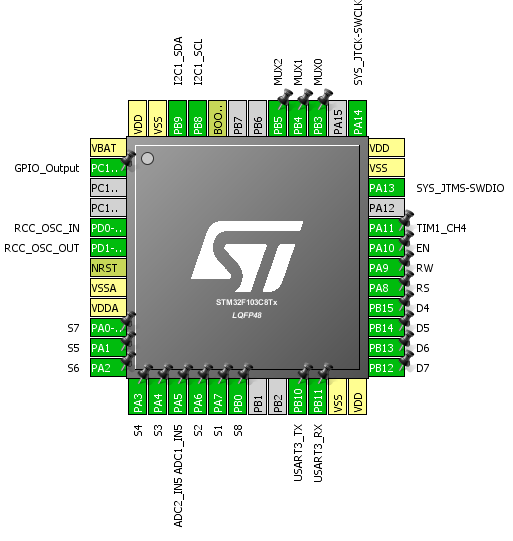
\includegraphics[scale=0.7]{imagens/pinagem_microcontrolador}
	\caption*{Fonte: Autoria Própria.}

\end{figure}

Como o microcontrolador proposto para este trabalho possui uma frequência de \textit{clock} maior que aquele utilizado por \citeonline{RUANI}, foi necessário descobrir a frequência de \textit{clock} ideal para alimentar as bobinas geradoras. Utilizando um \textit{software} chamado STM32Studio, pelo qual é possível monitorar variáveis em tempo real pelo computador, foi monitorada uma bobina sensora para alcançar o seu valor máximo quando o mais próximo possível da bobina geradora. Para isso, foi feito um pequeno teste com cada par sensor/gerador variando a frequência na bobina geradora de 95 $kHz$ até 105 $kHz$. Ao obter o valor máximo, este valor de frequência é deixado fixo para esse par.

\begin{figure}[H]
	\vspace{4mm}
	\centering
	\caption{Fluxograma que detalha a rotina desenvolvida para calibrar os sensores indutivos}
	\label{fig:fluxograma_calibragem_ind}
	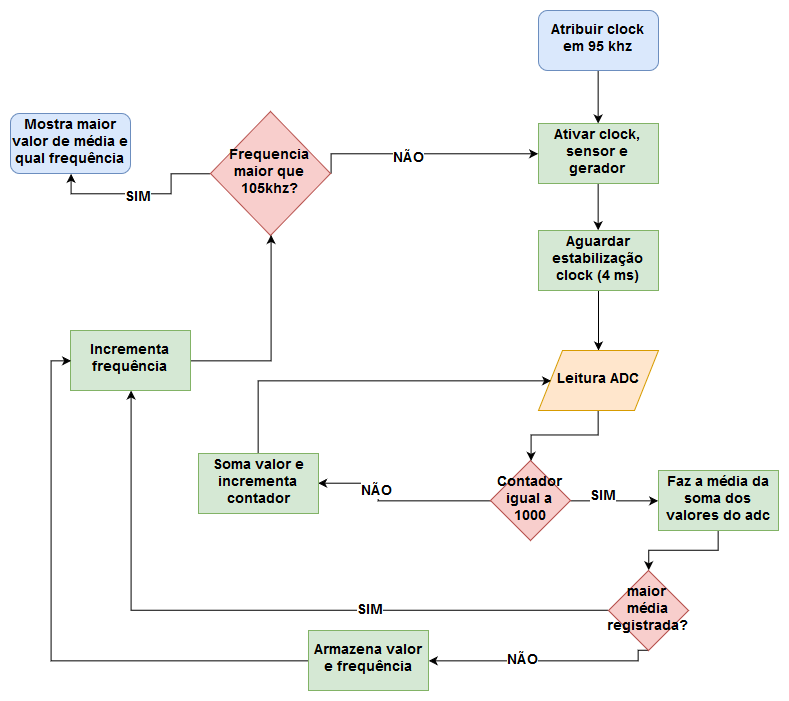
\includegraphics[scale=0.5]{imagens/calibrarIndutivo}	
	\caption*{Fonte: Autoria Própria.}
\end{figure}

Após configurados os valores para cada par sensor/gerador, foi feito o gesto que representa a letra A em LIBRAS, e o resultado obtido nos sensores indutivos pode ser observado no gráfico da Figura \ref{fig:sensores_letra_a}.

\begin{figure}[H]
	\vspace{4mm}
	\centering
	\caption{Valor dos sensores indutivos ao fazer o gesto da letra A em LIBRAS no software STM32Studio}
	\label{fig:sensores_letra_a}
	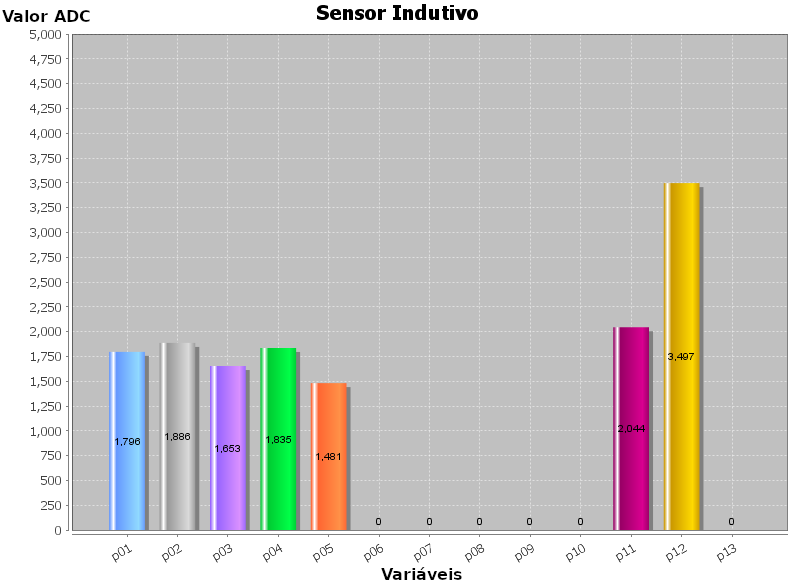
\includegraphics[scale=0.7]{imagens/LETRA_A_STMSTUDIO}
	\caption*{Fonte: Autoria Própria.}
\end{figure}

A relação de sensores e geradores com as variáveis exibidas na Figura \ref{fig:sensores_letra_a} é exibida na Tabela \ref{tab:relacao_sgv}.

\begin{table}[H]
	\vspace{4mm}
	\centering
	\caption{Relação de sensores e geradores com as variáveis da Figura \ref{fig:sensores_letra_a}}
	\label{tab:relacao_sgv}
	\resizebox{\textwidth}{!}{%
		\begin{tabular}{|l|l|l|l|l|l|l|l|l|l|l|l|l|l|}
			\hline
			\textbf{Variável} & p01 & p02 & p03 & p04 & p05 & p06 & p07 & p08 & p09 & p10 & p11 & p12 & p13 \\ \hline
			\textbf{Sensor} & S1 & S2 & S3 & S4 & S5 & S5 & S1 & S2 & S3 & S6 & G4 & G5 & G6 \\ \hline
			\textbf{Gerador} & G1 & G1 & G1 & G1 & G1 & G2 & G3 & G3 & G3 & G3 & S6 & S7 & S8 \\ \hline
		\end{tabular}%
	}
	\vspace{4mm}
	\caption*{Fonte: Autoria Própria.}
\end{table}

Na Figura \ref{tab:relacao_sgv} percebe-se que a medida p13 não está marcando um valor válido. Isso se deve ao fato do sensor/gerador terem dado defeito constantemente. Então foi analisada a necessidade deste sensor e foi decidido não utilizá-lo.
A rotina para a coleta dos dados de cada par sensor/gerador tem o funcionamento descrito pelo fluxograma da Figura \ref{fig:fluxograma_rotina_coleta}.
\begin{figure}[H]
	\vspace{4mm}
	\centering
	\caption{Fluxograma que detalha o funcionamento da rotina de coleta de dados do sensor indutivo.}
	\label{fig:fluxograma_rotina_coleta}
	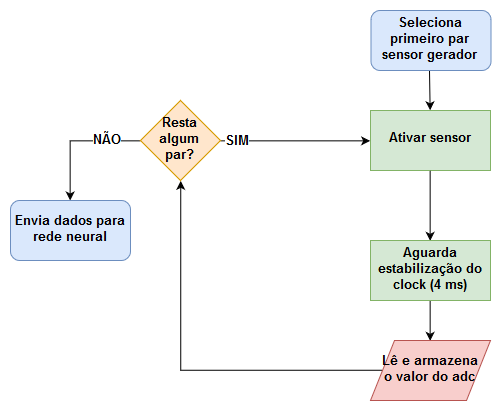
\includegraphics[scale=0.6]{imagens/rotinaColetaIndutivo}
	\caption*{Fonte: Autoria Própria.}
\end{figure}

A implementação da rotina de coleta de dados é exibida no Codigo \ref{cod:Indutivo}.

Após toda a codificação, foi testado o funcionamento com os mesmos valores da rede neural que foi implementada no trabalho anterior desenvolvido por \citeonline{RUANI}. Ao retirar um dos sensores indutivos, a entrada da rede neural implementada pelo \citeonline{RUANI} teria uma resposta errada, sendo. Considerando isto e também a diferença de periférico ADC do microcontrolador MSP430, utilizado no trabalho anterior, para o ADC do microcontrolador deste trabalho (STM32F103), foi decidido modificar a rede neural.

Porém, a resposta não estava satisfatória, devido a diferença dos periféricos A/D de um microcontrolador para outro. Então foi decidido refazer a rede neural.

O laço principal do \textit{firmware} é demonstrado no Código \ref{cod:mainloop}, onde é feita a coleta dos sensores indutivos, enviado para serial caso solicitado, e classificada a letra.

Para a implementação do \textit{display}, foi feito um código baseado na implementação de \cite{gihutDisplay}.

\subsection{Placa de adaptação para novo microcontrolador}
Para não refazer a placa toda, foi feita uma placa de adaptação para o novo microcontrolador, que possui como única função encaixar na placa de processamento de sinais e direcionar os pinos para os pinos corretos do stm32.

\begin{figure}[H]
	\vspace{4mm}
	\centering
	\caption{Vista das ligações da placa de adaptação para o microcontrolador stm32f103c8t6}
	\label{fig:placa2}
	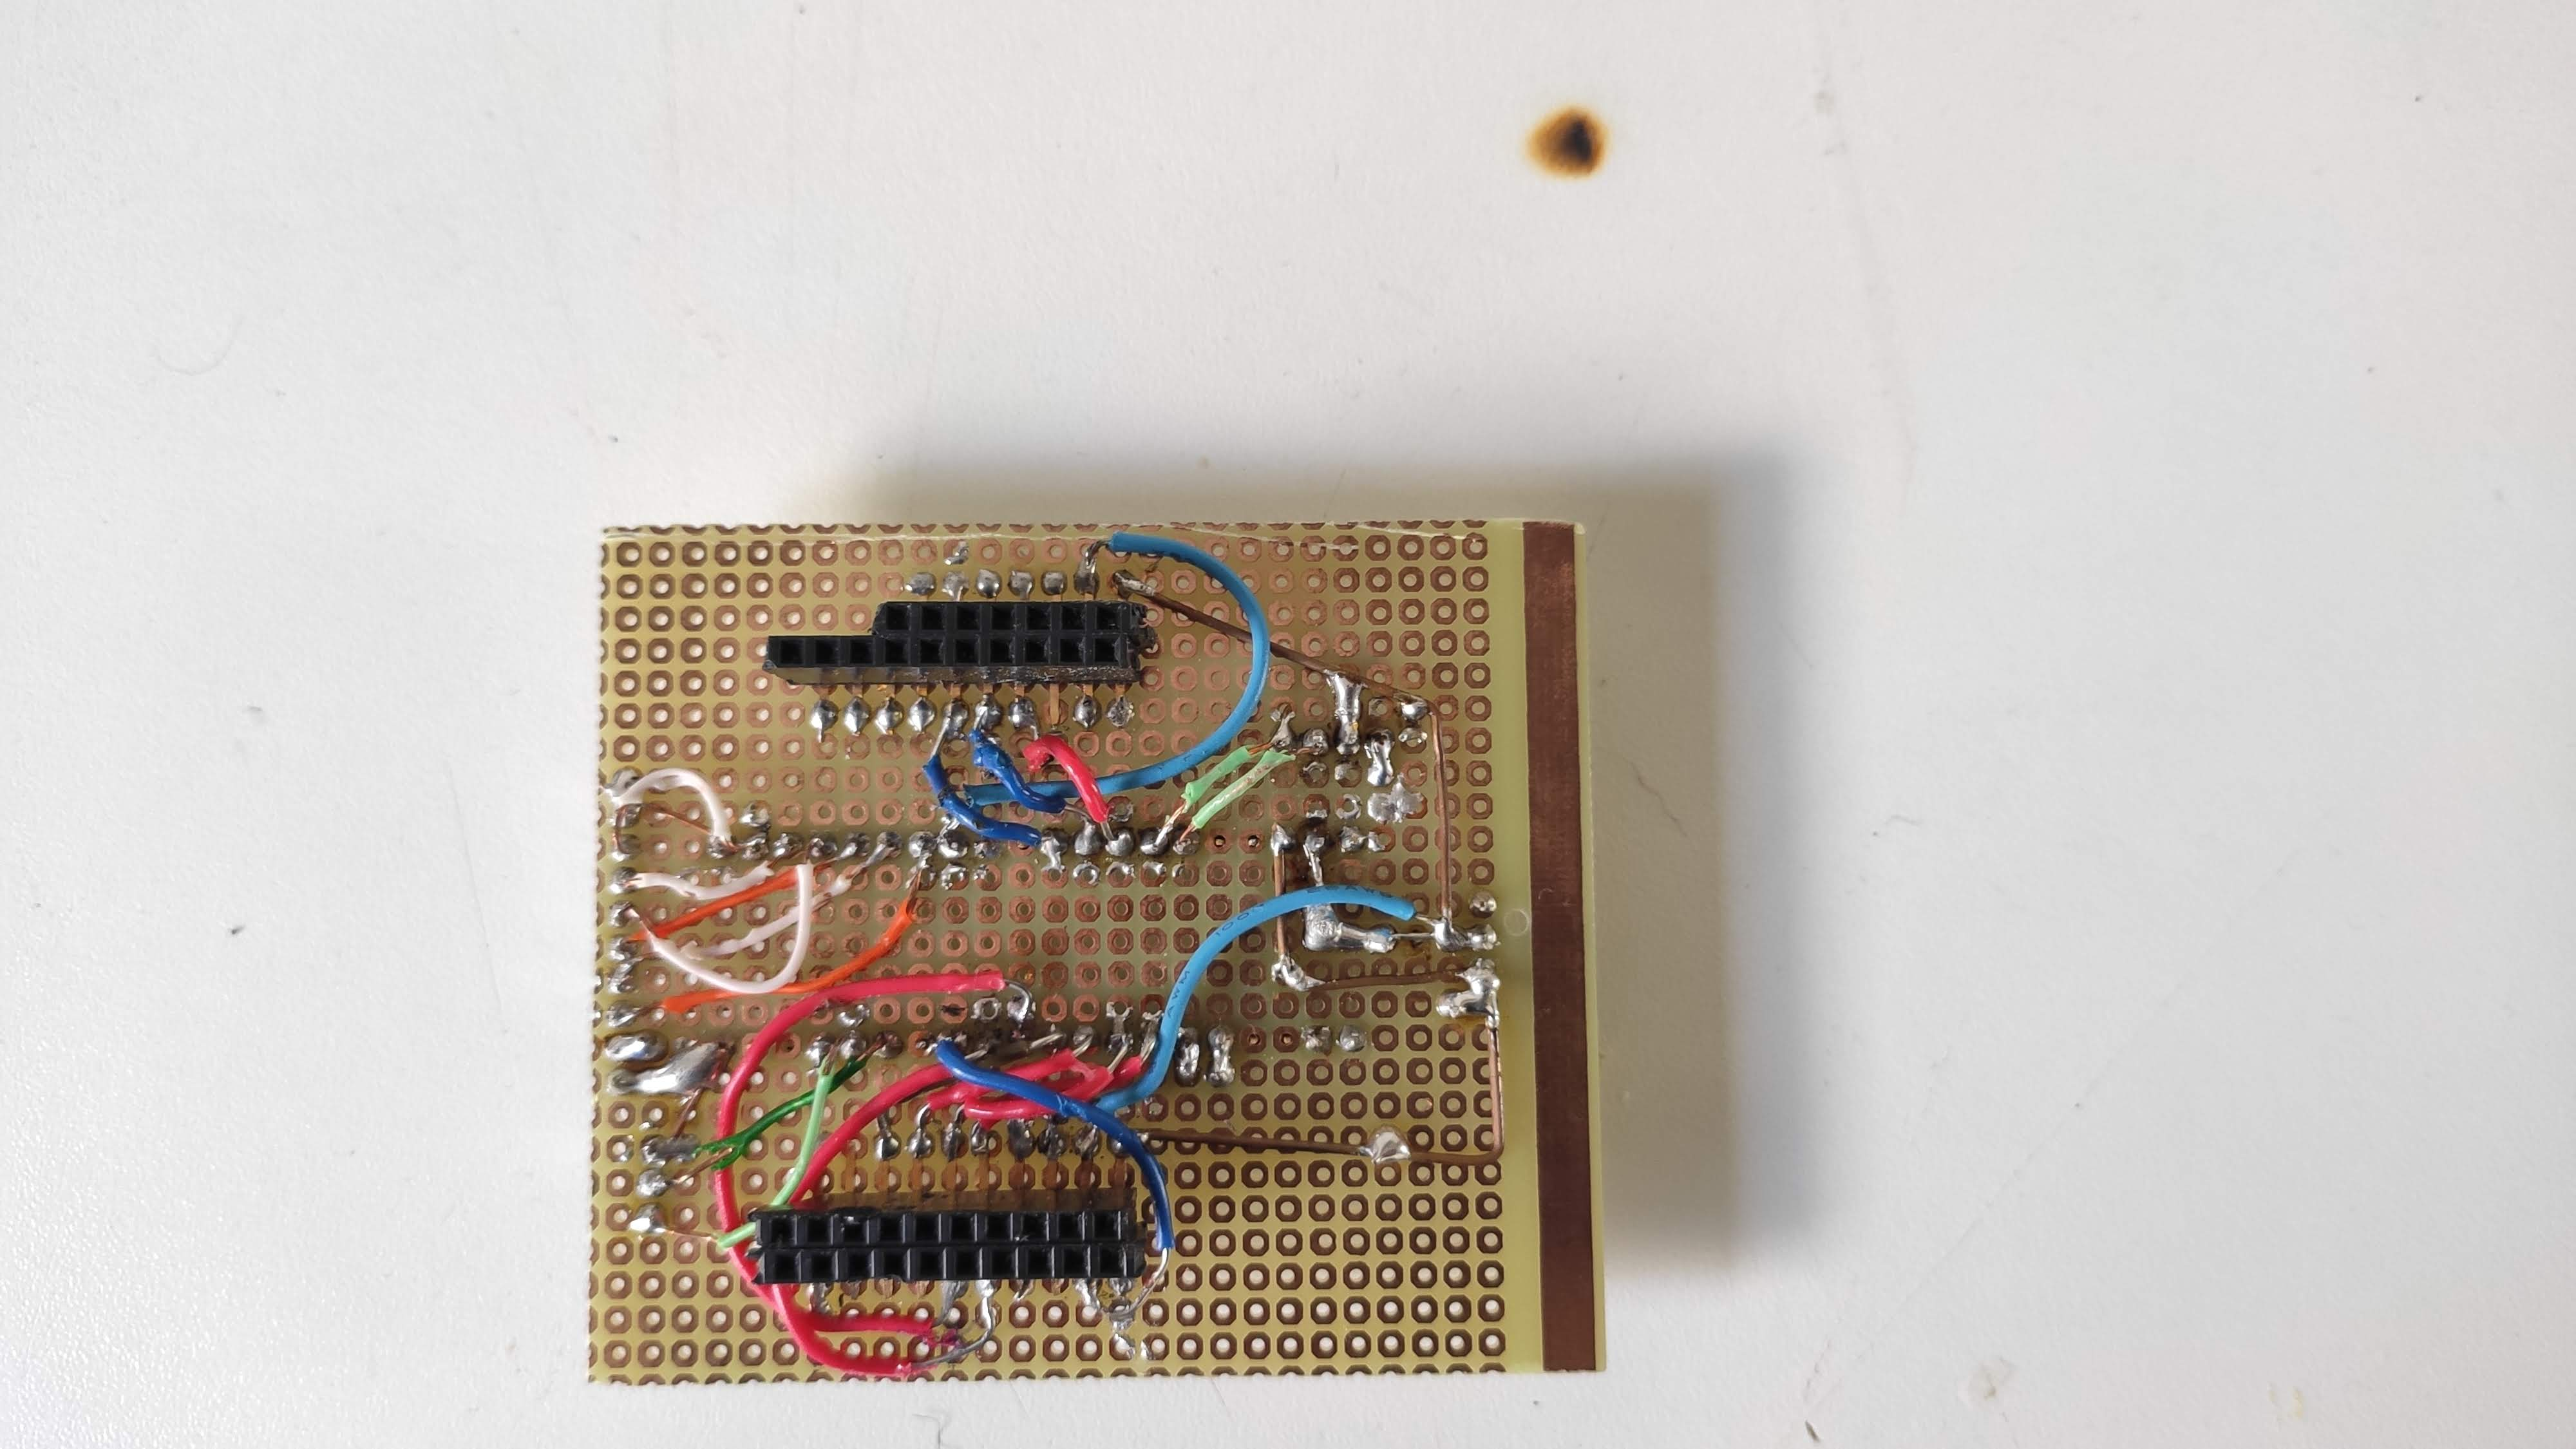
\includegraphics[scale=0.12, trim={20cm 2cm 45cm 15cm}, clip]{imagens/placa2}
	\caption*{Fonte: Autoria Própria.}
\end{figure}
Como demonstrado nas Figura \ref{fig:placa2}, a placa foi feita a partir de uma placa ilhada de contatos pela facilidade de fazer as ligações sem precisar de muito planejamento e software para produzi-la.

O posicionamento dos componentes da placa pode ser visto na Figura \ref{fig:placa1}. A placa conta com barras de pinos para ligar o \textit{display}, barra de pinos para conectar a interface serial e comunicar com o computador, barra de pinos para conectar o sensor inercial MPU6050, e também a barra de pinos para a alimentação das placas.

\begin{figure}[H]
	\vspace{4mm}
	\centering
	\caption{Vista de cima da placa de adaptação para o microcontrolador stm32f103c8t6}
	\label{fig:placa1}
	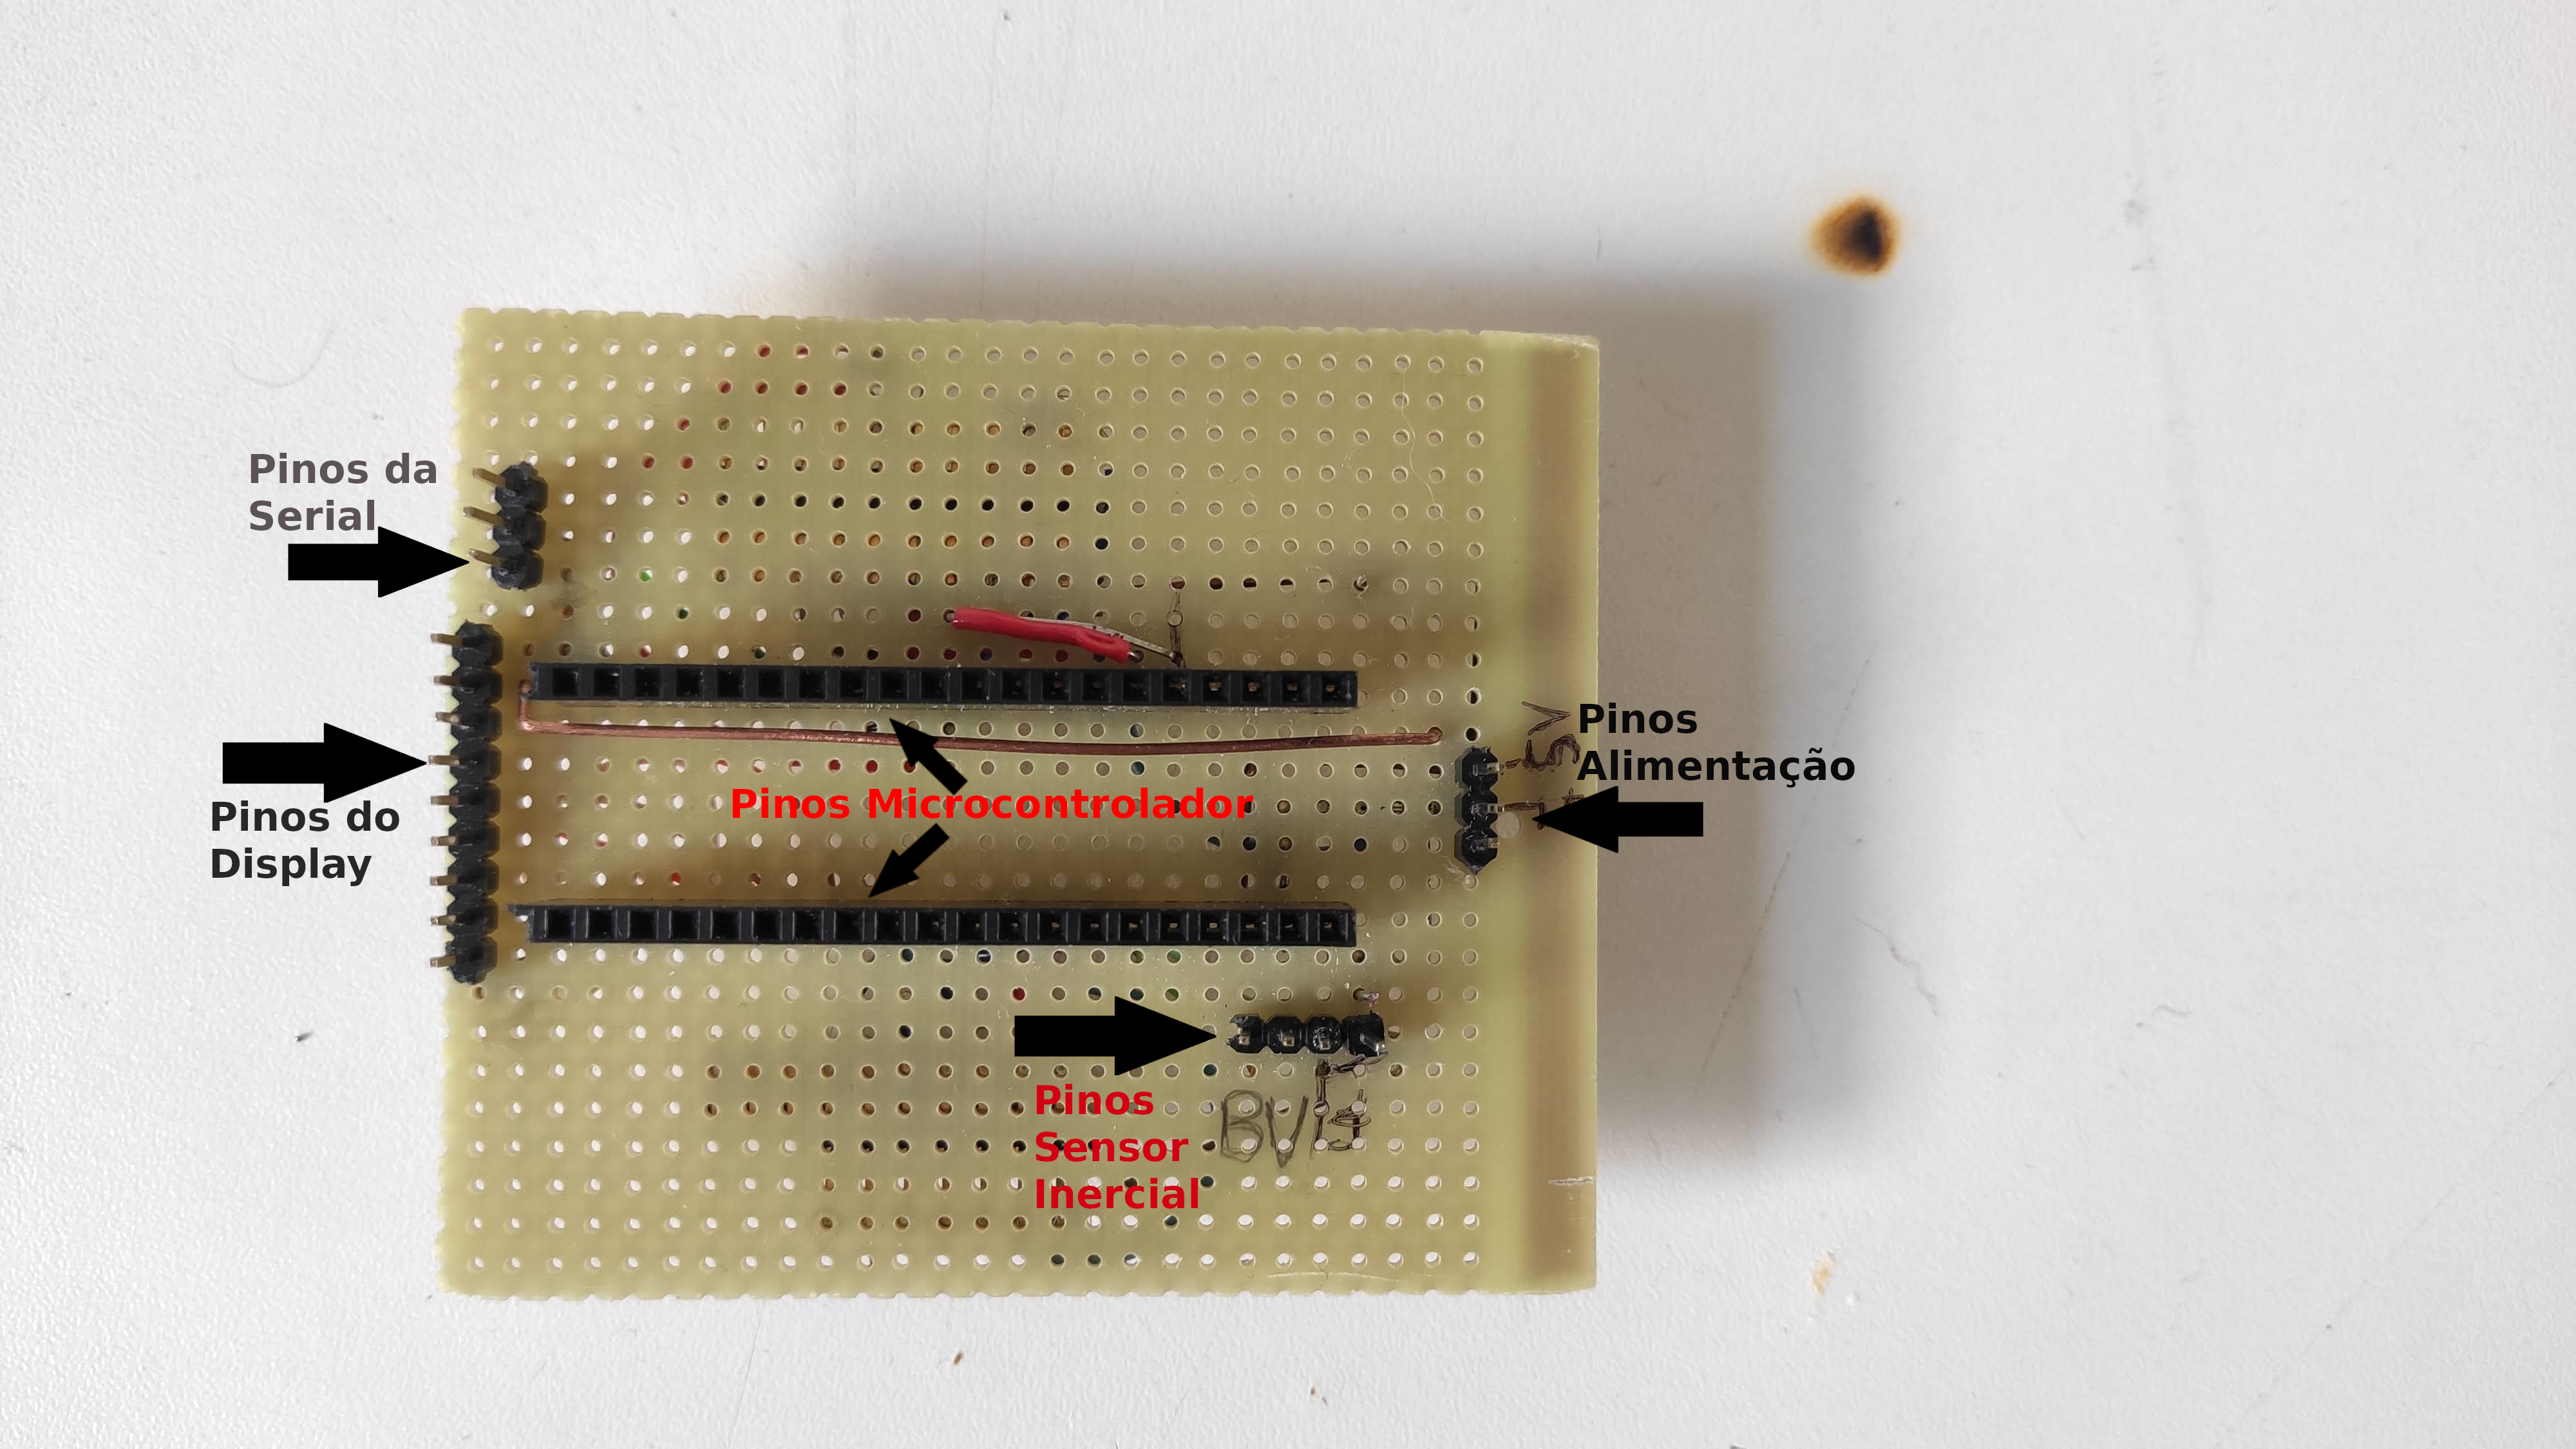
\includegraphics[scale=0.5, trim={2.5cm 3cm 8cm 4cm}, clip]{imagens/placa1}	
	\caption*{Fonte: Autoria Própria.}
\end{figure}

\subsection{Configuração sensor MPU6050 e Processamento de sinais}
Está sessão detalha a configuração do sensor MPU6050 e explica como foi feita o processamento dos sinais vindos do sensor. 	
\subsubsection{Configuração e calibração do sensor MPU-6050}
O sensor inercial, utilizando comunicação de circuitos inter-integrados ou I²C, sendo necessário o uso e configuração de uma interface serial neste padrão no microcontrolador.

 A biblioteca de abstração de hardware (HAL) disponibilizada pela fabricante do microcontrolador facilita a configuração de periféricos, necessitando apenas de poucas funções para configurar. Utilizando o \textit{datasheet} do sensor MPU6050, foi identificada a sequência de passos para iniciar, calibrar e ler os valores. Para calibrar o acelerômetro, são estimados os valores de \textit{offsets} necessários para o funcionamento do sensor. Esses valores variam para cada placa fabricada. Então foi desenvolvida uma rotina de calibração para o sensor. O sensor deve ser posicionado em uma superfície plana com o eixo Z em 90 graus com a superfície, como é exibido na Figura \ref{fig:MPU_Calb}.

\begin{figure}[H]
	\vspace{4mm}
	\centering
	\caption{Posicionamento da MPU6050 e seus eixos para a calibração}
	\label{fig:MPU_Calb}
	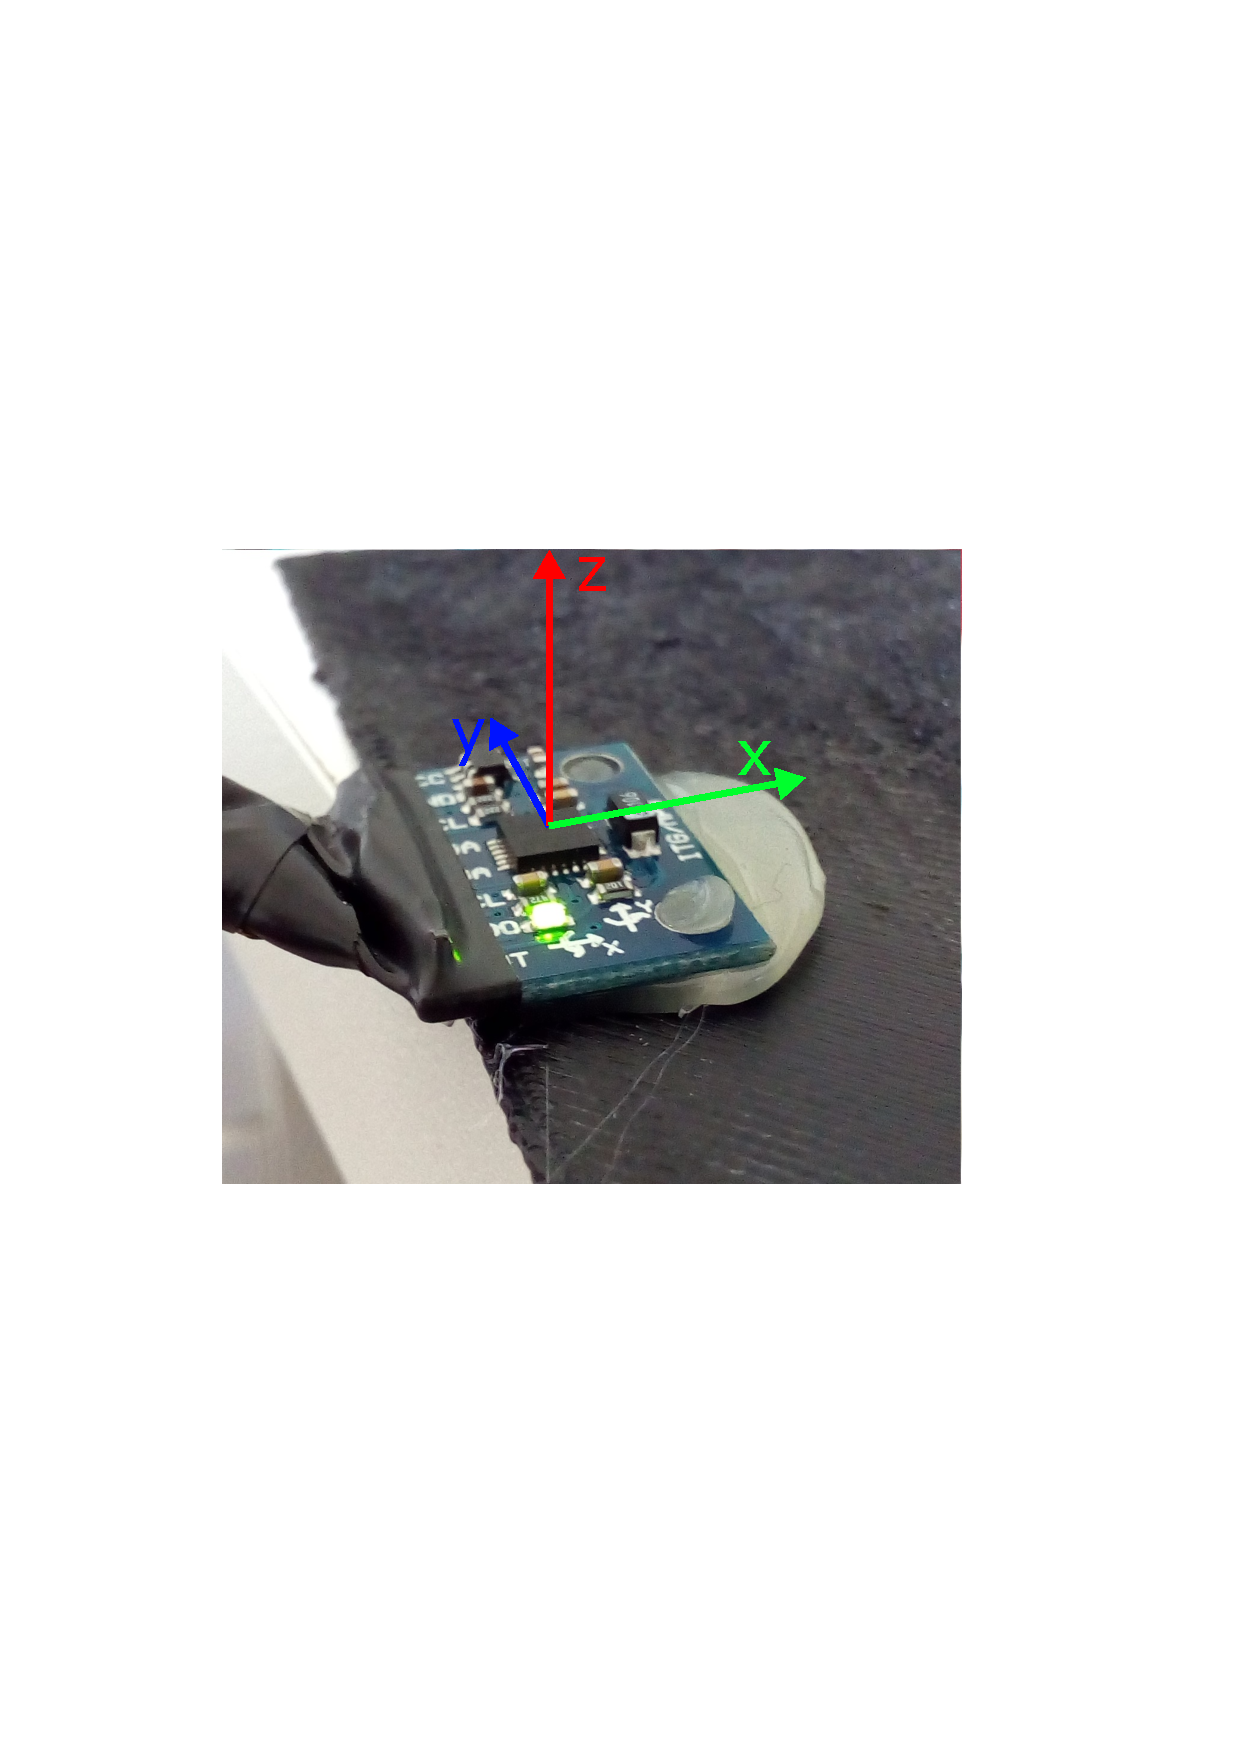
\includegraphics[scale=0.7, trim={5cm 10cm 7cm 9.3cm}, clip]{imagens/mpu_calib.pdf}
	\caption*{Fonte: Autoria Própria.}
\end{figure}

Para este trabalho, foi utilizado somente o acelerômetro para a detecção dos movimentos.

\subsubsection{Letras conflitantes e processamento dos sinais}
Observando todas as letras do alfabeto de LIBRAS (Figura \ref{fig:alfabeto}), nota-se que algumas letras tem o mesmo posicionamento de mãos, sendo apenas diferenciadas pelo movimento. Essas são: J e I; P, K e H; e X e Z; No trabalho anterior desenvolvido por \citeonline{RUANI}, foram deixadas de fora as letras com movimento (X, K, H, e J). Para reconhecer todas as letras, foi utilizado o acelerômetro para detecção de movimento.
Ao incluir detecção de movimento, as letras que contém a mesma posição de mão, como as letras J e I, tornam-se conflitantes, mesmo que a letra I não contenha movimento, porque a posição de mão dela é igual ao da letra J. O mesmo ocorre com as letras P, K, e H, onde a letra P não contém movimento e as letras H e K usam movimento.

 O trabalho do acelerômetro do sensor inercial é detectar esse movimento ocorrido. Na Figura \ref{fig:letrasMov}, são exibidas apenas as letras com movimentação. Posicionando o eixos de coordenadas do sensor inercial na luva como demonstrado na Figura \ref{fig:LuvaMPU}.

\begin{figure}[H]
	\vspace{4mm}
	\centering
	\caption{Posicionamento do sensor inercial na luva com eixo de coordenadas.}
	\label{fig:LuvaMPU}
	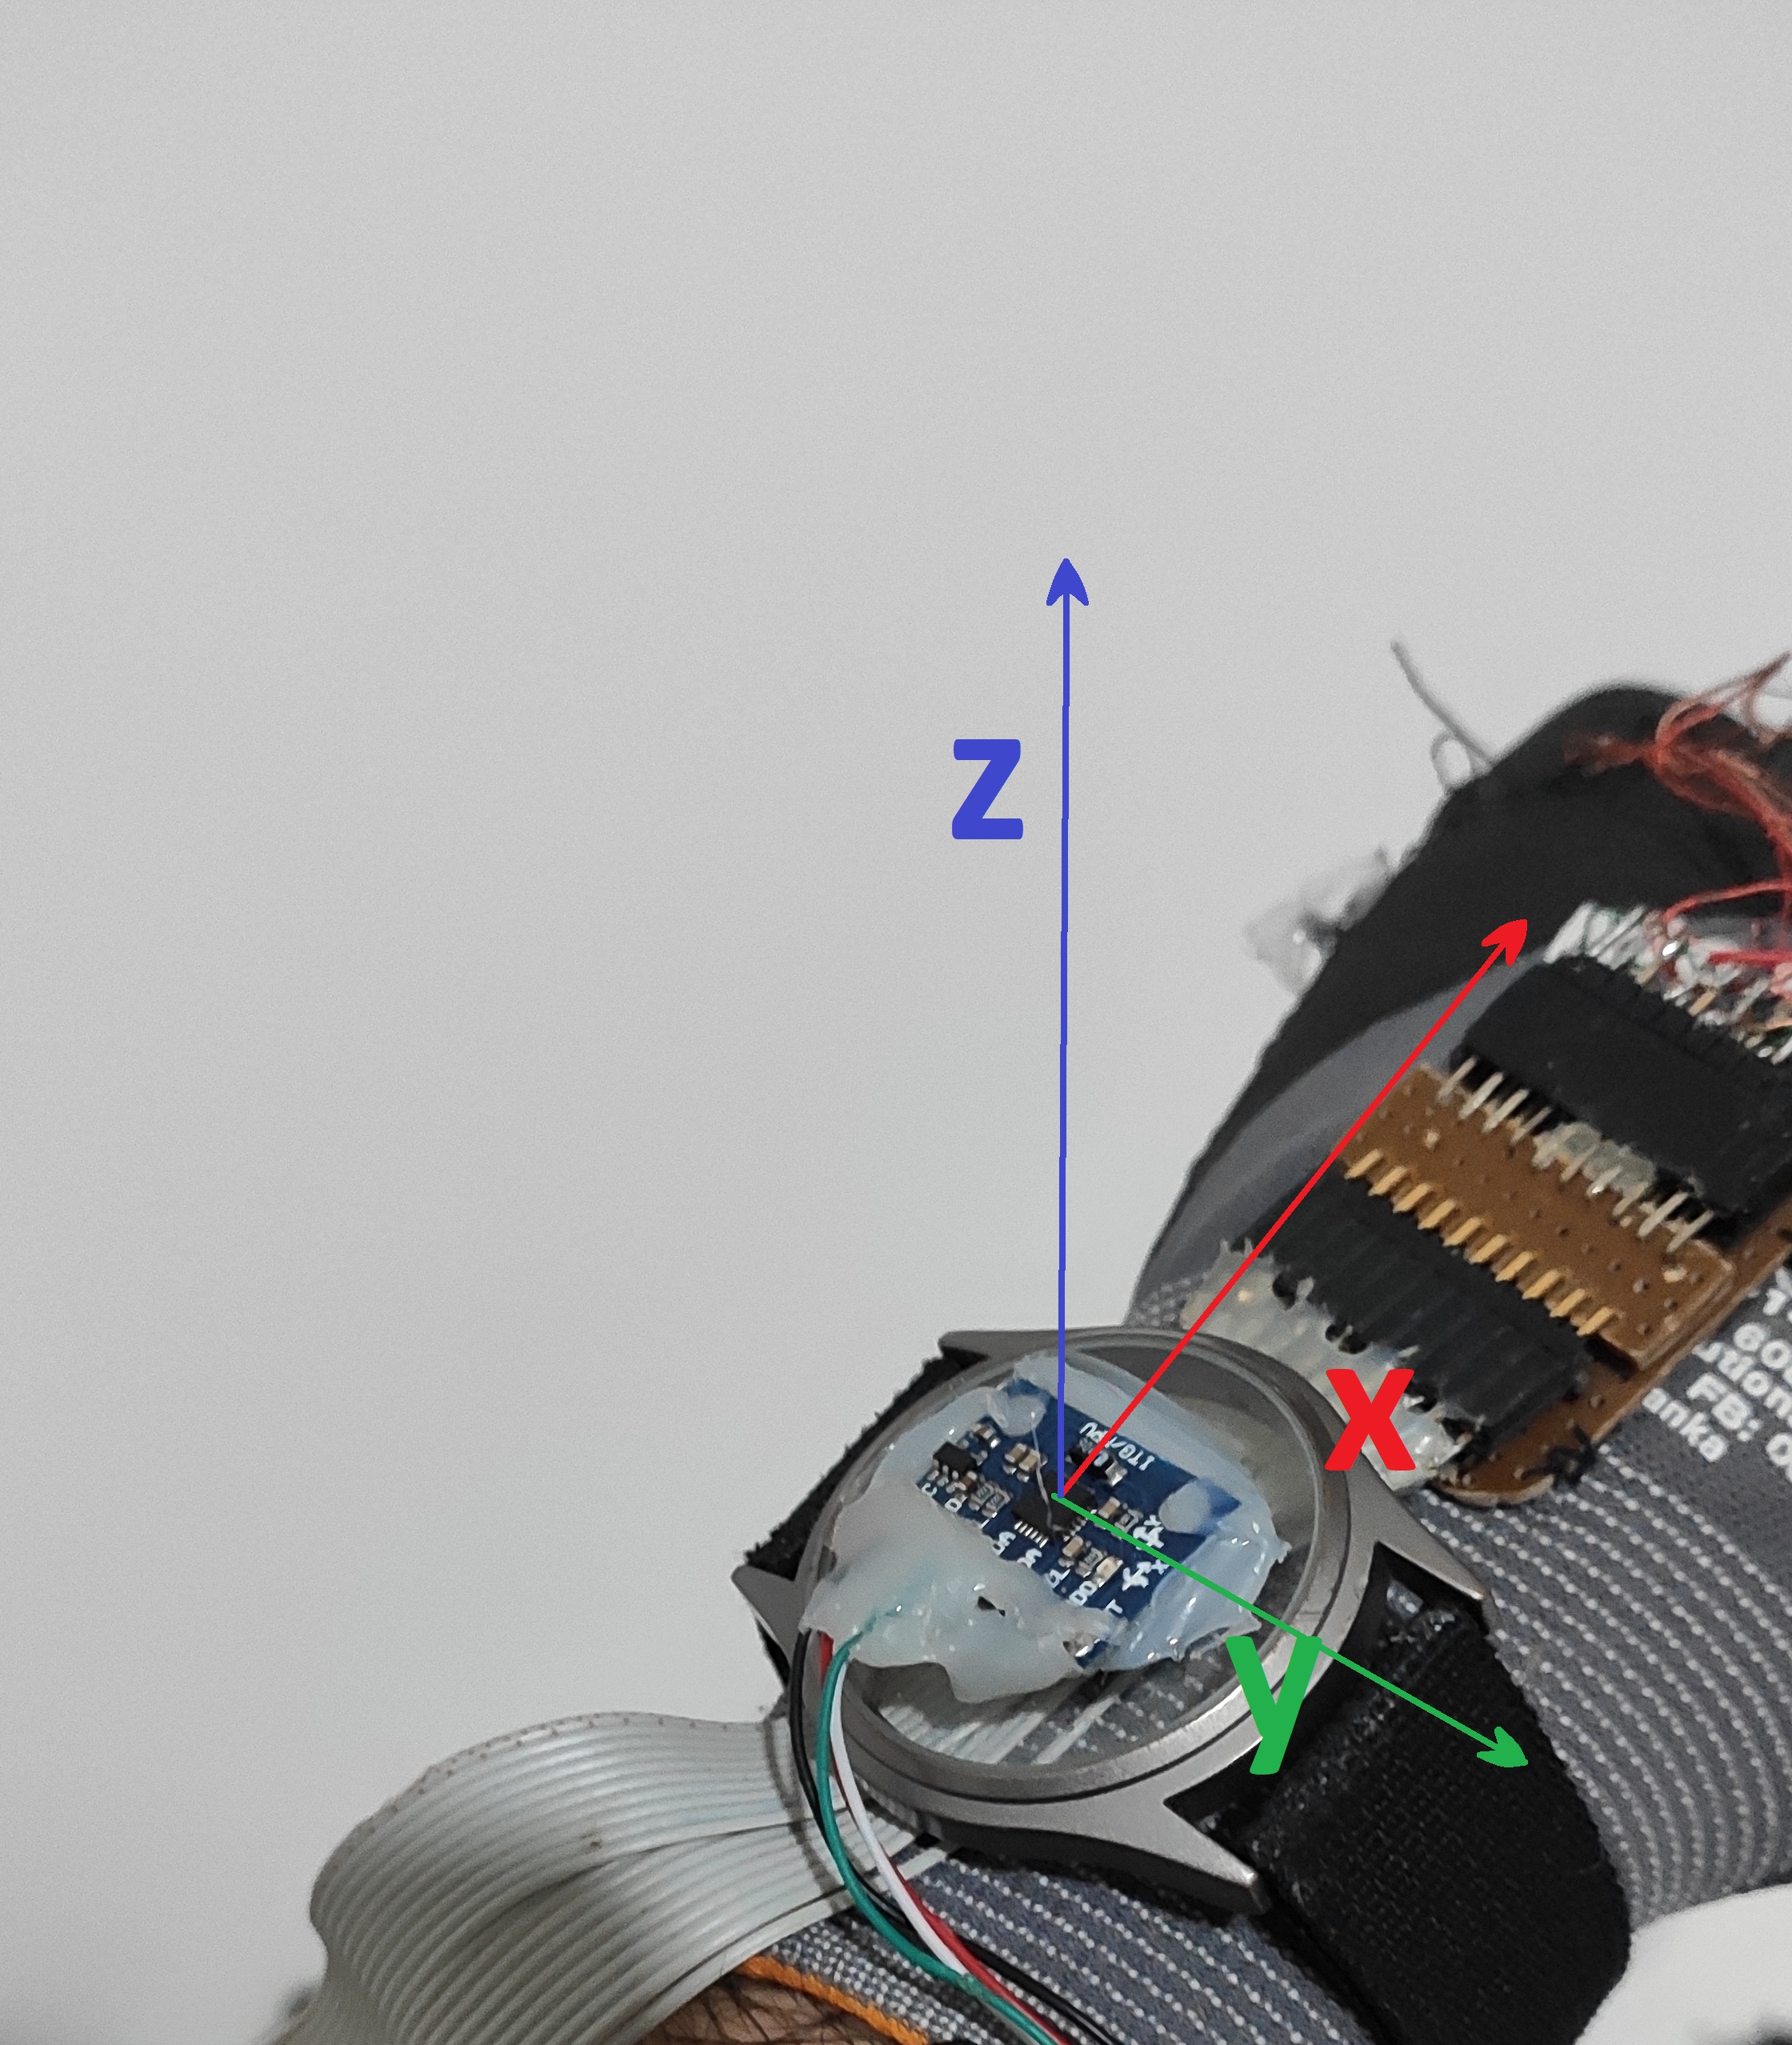
\includegraphics[scale=0.1]{imagens/luvaComMput}
	\caption*{Fonte: Autoria Própria.}
\end{figure}

Para detectar os movimentos das letra exibidas na Figura \ref{fig:letrasMov}, foram utilizadas as 3 coordenadas do acelerômetro ($x, y,$ e $z$), e a coordenada de rotação Roll.

\begin{figure}[H]
	\vspace{4mm}
	\centering
	\caption{Letras do alfabeto de libras que contém movimento.}
	\label{fig:letrasMov}
	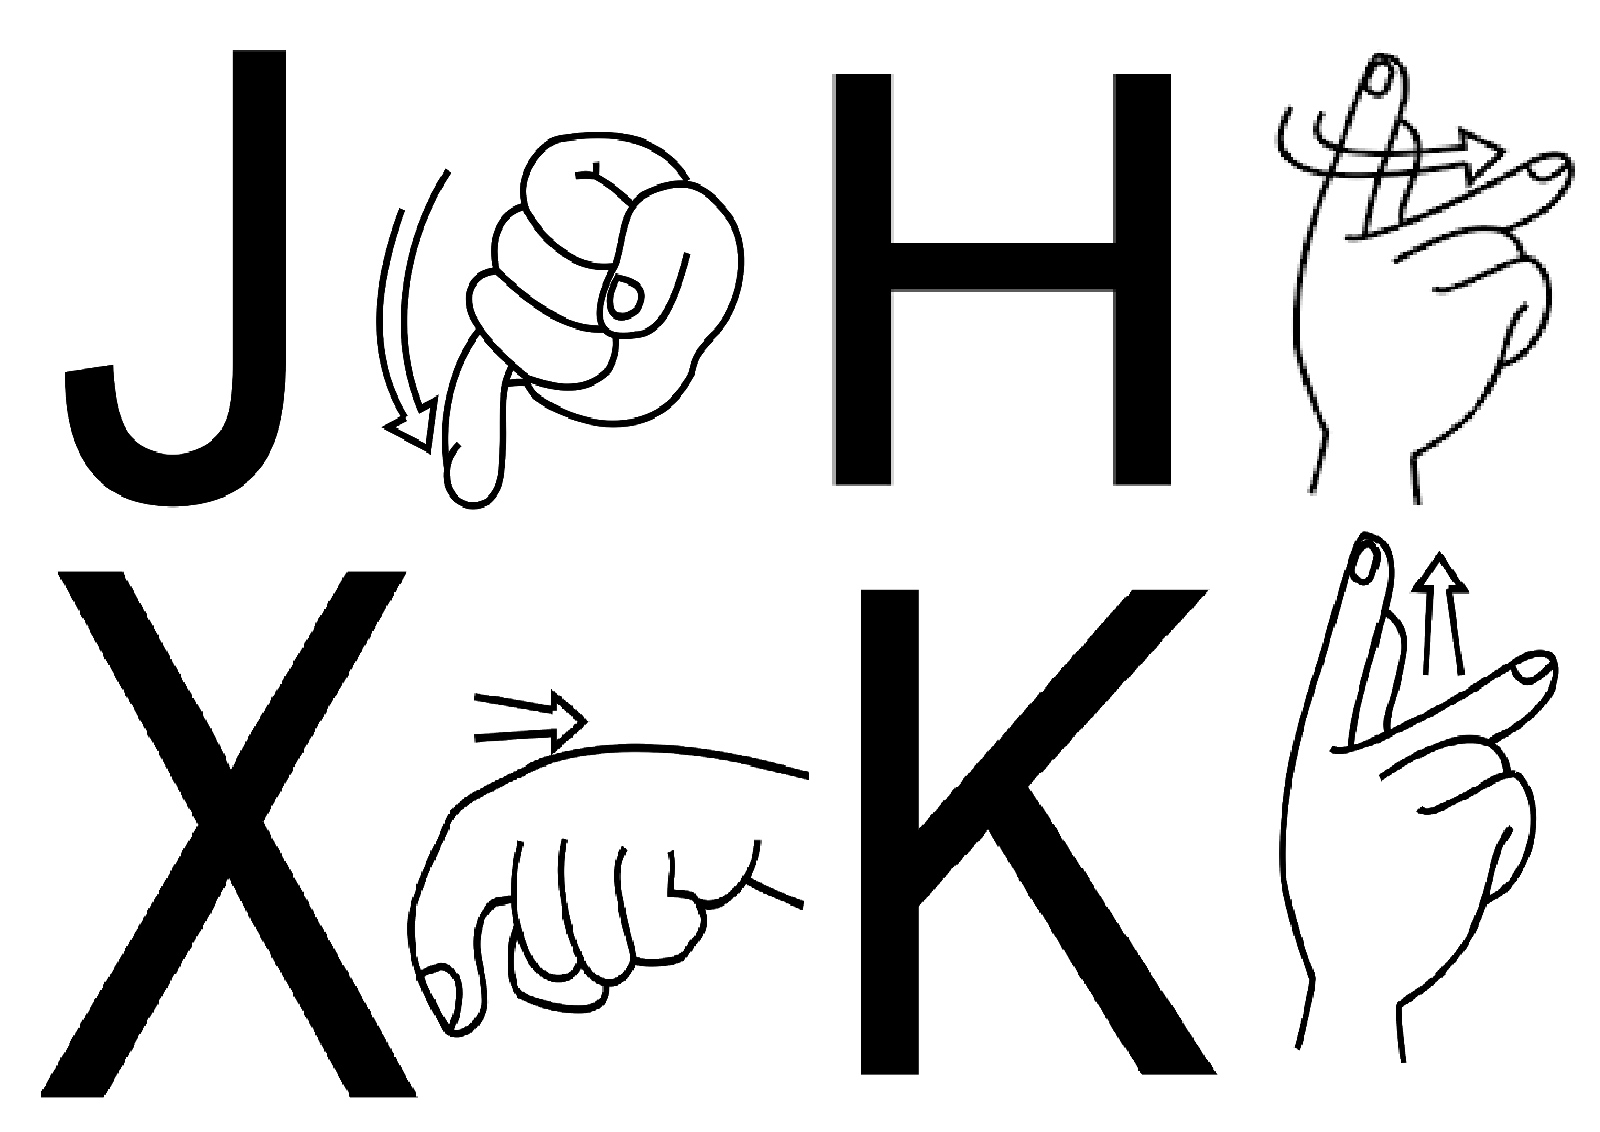
\includegraphics[scale=0.2]{imagens/letras_movimento}	
	\caption*{Fonte: Autoria Própria.}
\end{figure}

Os sinais provenientes da luva são os doze pares sensor/gerador. O sinal lido das bobinas pelo ADC já está processado, somente necessitando normalizar. E também os sinais vindos do acelerômetro.

Para captar o movimento, foi definido uma janela de tempo de $500$ $ms$, que é o tempo necessário para fazer o movimento de uma letra. Na Figura \ref{fig:espec_ACC} pode ser visto os sinais do acelerômetro no período de $500$ $ms$.

\begin{figure}[H]
	\vspace{4mm}
	\centering
	\caption{Gráficos dos sinais do acelerômetro, amostrando $500$ $ms$.}
	\label{fig:espec_ACC}
	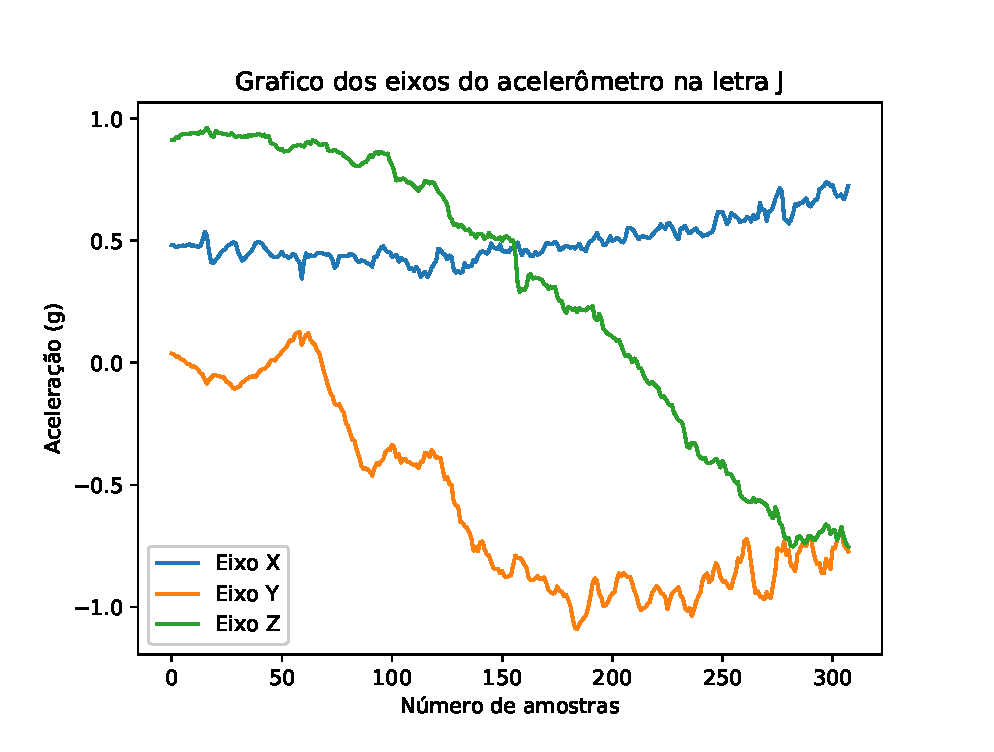
\includegraphics[scale=0.45]{imagens/espectro_acc.eps}
	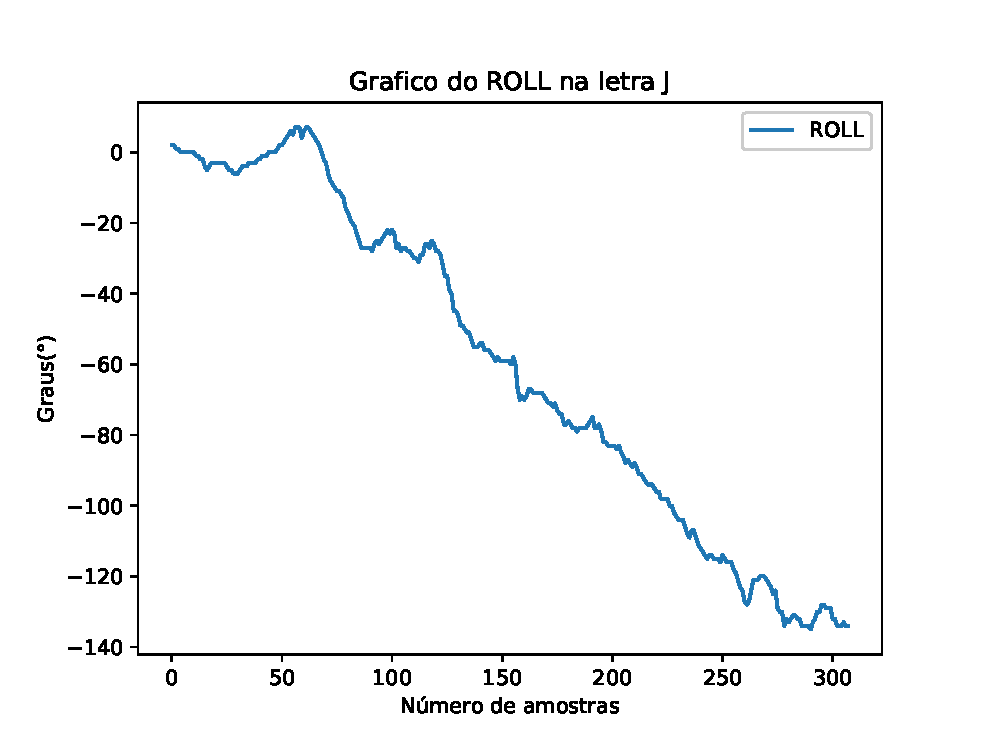
\includegraphics[scale=0.45]{imagens/roll_acc.eps}	
	\caption*{Fonte: Autoria Própria.}
\end{figure}

Essa janela de tempo é dividida em 10 pedaços, e a cada $50$ $ms$, são coletados os dados dos eixos do sensor inercial, e sempre a amostra mais velha dos dados é descartada, fazendo com que a janela de $500$ $ms$ deslize no tempo. Um exemplo de como será a janela pode ser visto na Figura \ref{fig:janela}.

\begin{figure}[H]
	\vspace{4mm}
	\centering
	\caption{Janela de amostras}
	\label{fig:janela}
	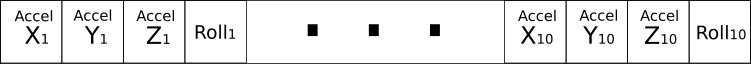
\includegraphics[scale=0.7]{imagens/janela.png}
	\caption*{Fonte: Autoria Própria.}
\end{figure}

\subsection{Redes Neurais Implementadas}

Para manter o foco na solução sugerida por este trabalho, foram separadas as letras em dois grupos: letras sem conflito, e as letras conflitantes.
As letras sem conflito são aquelas que somente o sensor indutivo consegue classificar, sem a necessidade do sensor inercial. E as letras conflitantes são as quais tem a necessidade de utilizar o sensor inercial como diferencial entre elas. As letras consideradas conflitantes são P, H, K, I, J, Z, X.
Considerando esses dois grupos, foram feitas duas redes neurais. A posição de mão das letras conflitantes entram na classificação das não conflitantes, mas só é exibido um resultado quando é executada a segunda classificação com os dados do sensor inercial.

\subsubsection{Rede Neural para os sensores indutivos}
Como já mencionado na subseção \ref{sec:transf}, a rede neural que trata dos sinais provenientes dos sensores indutivos (pares de bobinas sensora/geradora) foi refeita, ao retirar um dos sensores indutivos, uma das entradas sempre será zero afetando o desempenho do sistema.

As características são bem definidas como sendo cada par de bobinas sensora/geradora da luva. Foi criada um Perceptron Multi Camada (MLP) com 21 neurônios de camada oculta, utilizando a função de ativação tangente hiperbólica (Sessão \ref{sec:funcao}). 

O treinamento foi feito com um conjunto de 50 amostras de cada letra, onde 75\% para treinamento e 25\% para teste da rede. Esse processo de divisão dos dados é feito com uma mistura na ordem dos dados. Para permanecer parecida com a rede implementada no trabalho anterior, foi utilizada a mesma quantia de neurônios de camada oculta (21 neurônios).

O código \ref{cod:rede1} foi elaborado para o treinamento, obtendo uma taxa de acerto de 96,36\% ao final do treinamento e teste. \hspace{20pt}

Os dados dos sensores de cada letra feita foi armazenada em arquivos, e a função arruma\_dados é responsável por juntar esses dados em uma matriz de características. Após as características são redimensionadas para ficar no intervalo da função de ativação de $[-1, 1]$. Após isso é feita a divisão dos dados em vetores de teste e treino, (x\_train e x\_test). Então é feito o treino chamando a função \textit{fit} do \textit{MLPClassifier}. O resultado da classificação é visualizado com a função \textit{predict}, na qual usa o vetores de teste para comparar a classificação feita pela rede e a resposta real.

Para efetivamente fazer a classificação, é implementado o método \textit{feedfoward}, utilizando os pesos obtidos no treinamento. Resultando no Código \ref{cod:feedforward1}.

Após a classificação, para transformar o número em uma letra é utilizada uma função de pós-processamento descrita no Código \ref{cod:pos1}.

Nas letras de retorno pode-se notar os números 1, 2, e 3. Essas são as classes de pose de mão que são das letras conflitantes, esse é a ligação com a outra rede neural implementada, ou seja, não são exibidos esses números no \textit{display}.

\subsubsection{Rede Neural sensor inercial}
Considerando os dados já processados, foram colhidos pela serial e inseridos no código em Python para treinamento da rede. As características
são elas que são 10 pedaços de tempo em que cada pedaço tem 4 valores. Foram colhidos 25 amostras de cada movimento, incluindo uma posição sem movimento. No Código \ref{cod:rede2}, está demonstrado o treinamento da rede responsável pelo acelerômetro. Foi utilizado a função de ativação tangente hiperbólica. Utilizando 80 \% dos dados para treino e 20 \% para teste separados aleatoriamente.
 
 
A função \textit{LoadFromCsv} carrega os amostras dos arquivos e reúne em um vetor de características. Então esses dados são redimensionados para se adequar a função de ativação que é o intervalo de $[-1, 1]$. Então são separados os conjuntos de treino e teste para executar a função \textit{fit} que treina a rede neural. A função \textit{predict} compara os valores reais de classificação com os valores classificados e retorna o valor de acerto da rede treinada.

A função de \textit{feedfoward} implementada é a mesma do Código \ref{cod:feedforward1}, mudando apenas o pesos. O pós-processamento também só alterando o vetor de classes de saída que são as do Código \ref{cod:feedfor2}.

A função que faz a ligação das duas redes neurais é descrita no Código \ref{cod:classify}, onde são os dados do sensor indutivo são tratados e classificados. Caso a classificação seja uma das classes das letras conflitantes (1, 2, ou 3), então é acionado o acelerômetro para detectar o movimento e depois ele é classificado. No diagrama da Figura \ref{fig:fluxograma_trabalho_todo} está o detalhado o \textit{firmware} desenvolvido.
\begin{figure}[H]
	\centering
	\caption{Fluxograma que descreve o comportamento do \textit{firmware} a ser desenvolvido.}
	\label{fig:fluxograma_trabalho_todo}
	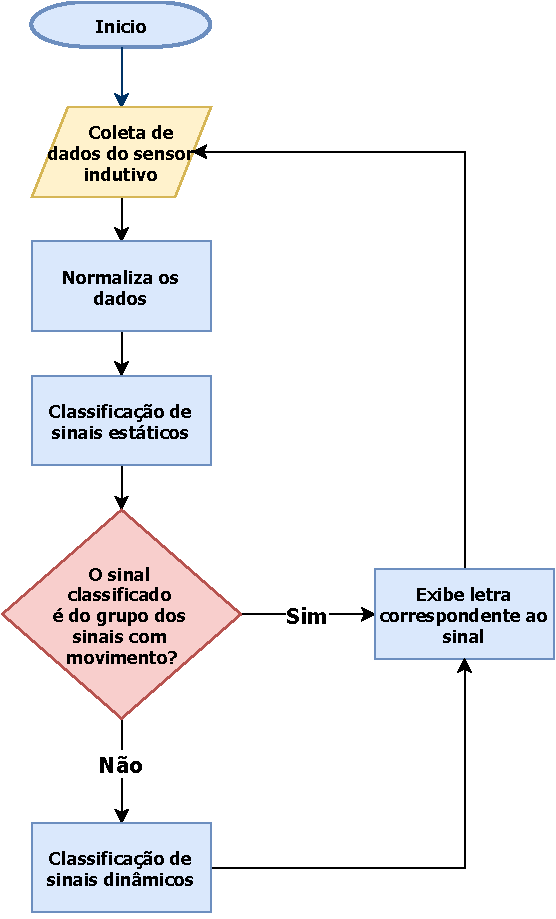
\includegraphics[scale=0.8]{imagens/fluxograma_trabalho_todo.pdf}	
	\caption*{Fonte: Autoria Própria.}
\end{figure}